\documentclass[page number,usenames,dvipsnames]{beamer}
\usetheme[sectionpage=none,numbering=fraction,progressbar=foot]{metropolis}

\usepackage{pgf,tikz}
\usetikzlibrary{arrows}
\usetikzlibrary{positioning,shapes,fit}
\usepackage{graphicx}
\usepackage{amsmath,amssymb,amsthm,textcomp}
\usepackage{proof}
\usepackage{listings}
\usepackage{xcolor}
\usepackage{pgf,tikz}
\usepackage{algorithm}
\usepackage{algpseudocode}
\usepackage{wrapfig}
\usetikzlibrary{calc,shapes.multipart,chains,arrows,positioning,shapes,tikzmark}
\usepackage{multicol}
\usepackage{btreecursor}
\usepackage{lstcoq}

\definecolor{spec}{HTML}{6F1616}
\definecolor{prog}{HTML}{106235}
\def\spec#1{{\color{spec}\textbf{#1}}}
\def\prog#1{{\color{prog}\textbf{#1}}}
\newcommand{\wand}{\mathrel{-\hspace{-.7ex}*}}

\lstset{language=C,
                basicstyle=\ttfamily\footnotesize,
                keywordstyle=\color{RedViolet}\ttfamily,
                stringstyle=\color{Violet}\ttfamily,
                commentstyle=\color{MidnightBlue}\ttfamily,
                morecomment=[l][\color{magenta}]{\#},
                morekeywords={Bool, Key, size_t},
                emph={%  
                  Relation_T, Cursor_T, BtNode_T, Relation, Cursor, BtNode, Entry, Child_or_Record%
                },emphstyle={\color{Maroon}}
}

\makeatletter
\makeatother

\setcounter{tocdepth}{1} % remove subsection from table of contents

% colors
\definecolor{mDarkRed}{HTML}{6F1616}
\definecolor{mDarkGreen}{HTML}{106235}
\definecolor{mTeal}{HTML}{112233}
\definecolor{mBlack}{HTML}{000000}
\setbeamercolor{normal text}{fg=mTeal}
\setbeamercolor{alerted text}{fg=mDarkRed}
\setbeamercolor{example text}{fg=mDarkGreen}
\setbeamercolor{title separator}{fg=purple,bg=mBlack}

\def\outline{
  \begin{frame}[plain,noframenumbering]
    \frametitle{Outline}
    \tableofcontents[currentsection]
  \end{frame}
}

\def\btree{B+Tree}
\def\btrees{B+Trees}
\def\todo#1{{\color{red}#1}}
\def\btrep{\texttt{btnode\_rep}}

\begin{document}
\title[shorttitle]{VST Verification of B+Trees with Cursors}

\author[Aur\`ele Barri\`ere]{Aur\`ele Barri\`ere}

\date{\textit{ENS Rennes}
  \vfill
  \textbf{Supervisor:} Andrew W. Appel\\
  \textit{Princeton University}
  \vfill
  \textbf{February 1st, 2018 - June 29th, 2018}
  \vfill}

%% BTree Style
\tikzstyle{btreeptr} = [draw, semithick, fill=blue!10, minimum height=2em]
\tikzstyle{btreeval} = [draw, semithick, fill=yellow!10, minimum size=2em]
\tikzstyle{btreevale} = [draw,semithick, fill=red!30!blue!15, minimum size=2em]
\tikzstyle{btlink} = [draw, semithick, ->, >=triangle 45]

\def\beforeinsert{
\begin{figure}
\makebox[\textwidth][c]{
  \scalebox{.5}{
    \begin{tikzpicture}
      % 
      \btreeinodefour{root}{20}{}{}{};
      \xyshift{-40mm}{-20mm}{\btreeinodefour{n1}{5}{9}{12}{15}}
      \xyshift{40mm}{-20mm}{\btreeinodefour{n2}{25}{30}{}{}}
      % 
      \xyshift{-130mm}{-40mm}{\btreelnodefour{n11}{0}{1}{2}{3}}
      \xyshift{-95mm}{-40mm}{\btreelnodefour{n12}{5}{6}{7}{8}}
      \xyshift{-60mm}{-40mm}{\btreelnodefour{n13}{9}{10}{11}{}}
      \xyshift{-25mm}{-40mm}{\btreelnodefour{n14}{12}{14}{}{}}
      \xyshift{10mm}{-40mm}{\btreelnodefour{n15}{15}{18}{}{}}
      \xyshift{45mm}{-40mm}{\btreelnodefour{n21}{20}{22}{23}{}}
      \xyshift{80mm}{-40mm}{\btreelnodefour{n22}{25}{27}{28}{}}
      \xyshift{115mm}{-40mm}{\btreelnodefour{n23}{30}{33}{34}{35}}
      % 
      \foreach \x in {1,2} { \btreelink{root-\x}{n\x} }
      \foreach \x in {1,2,3,4,5} { \btreelink{n1-\x}{n1\x} }
      \foreach \x in {1,2,3} { \btreelink{n2-\x}{n2\x} }
    \end{tikzpicture}
    
  }}
  \caption{A \btree}
  \label{bt}
  \end{figure}}


\def\afterinsert{
\begin{figure}
\makebox[\textwidth][c]{
  \scalebox{.5}{
    \begin{tikzpicture}
      % 
      \btreeinodefour{root}{9}{20}{}{};
      \xyshift{-60mm}{-20mm}{\btreeinodefour{n1}{2}{5}{}{}}
      \xyshift{-0mm}{-20mm}{\btreeinodefour{n2}{12}{15}{}{}}
      \xyshift{60mm}{-20mm}{\btreeinodefour{n3}{25}{30}{}{}}
      % 
      \xyshift{-165mm}{-40mm}{\btreelnodefour{n11}{0}{1}{2}{}}
      \xyshift{-130mm}{-40mm}{\btreelnodefour{n12}{3}{4}{}{}}
      \xyshift{-95mm}{-40mm}{\btreelnodefour{n13}{5}{6}{7}{8}}
      \xyshift{-60mm}{-40mm}{\btreelnodefour{n21}{9}{10}{11}{}}
      \xyshift{-25mm}{-40mm}{\btreelnodefour{n22}{12}{14}{}{}}
      \xyshift{10mm}{-40mm}{\btreelnodefour{n23}{15}{18}{}{}}
      \xyshift{45mm}{-40mm}{\btreelnodefour{n31}{20}{22}{23}{}}
      \xyshift{80mm}{-40mm}{\btreelnodefour{n32}{25}{27}{28}{}}
      \xyshift{115mm}{-40mm}{\btreelnodefour{n33}{30}{33}{34}{35}}
      % 
      \foreach \x in {1,2,3} { \btreelink{root-\x}{n\x} }
      \foreach \x in {1,2,3} { \btreelink{n1-\x}{n1\x} }
      \foreach \x in {1,2,3} { \btreelink{n2-\x}{n2\x} }
      \foreach \x in {1,2,3} { \btreelink{n3-\x}{n3\x} }
    \end{tikzpicture}
  }}
  \caption{\textbf{Fig.}~\ref{bt} after inserting a new record for key 4}
  \label{btinsert}
  \end{figure}
}


\def\cursor{
\begin{figure}
\makebox[\textwidth][c]{
  \scalebox{.5}{
    \begin{tikzpicture}
      % 
      \btreeinodefour{root}{20}{}{}{};
      \xyshift{-40mm}{-20mm}{\btreeinodefour{n1}{5}{9}{12}{15}}
      \xyshift{40mm}{-20mm}{\btreeinodefour{n2}{25}{30}{}{}}
      % 
      \xyshift{-130mm}{-40mm}{\btreelnodefour{n11}{0}{1}{2}{3}}
      \xyshift{-95mm}{-40mm}{\btreelnodefour{n12}{5}{6}{7}{8}}
      \xyshift{-60mm}{-40mm}{\btreelnodefour{n13}{9}{10}{11}{}}
      \xyshift{-25mm}{-40mm}{\btreelnodefour{n14}{12}{14}{}{}}
      \xyshift{10mm}{-40mm}{\btreelnodefour{n15}{15}{18}{}{}}
      \xyshift{45mm}{-40mm}{\btreelnodefour{n21}{20}{22}{23}{}}
      \xyshift{80mm}{-40mm}{\btreelnodefour{n22}{25}{27}{28}{}}
      \xyshift{115mm}{-40mm}{\btreelnodefour{n23}{30}{33}{34}{35}}
      % 
      \foreach \x in {1,2} { \btreelink{root-\x}{n\x} }
      \foreach \x in {1,2,3,4,5} { \btreelink{n1-\x}{n1\x} }
      \foreach \x in {1,2,3} { \btreelink{n2-\x}{n2\x} }
      %
      \xyshift{-120mm}{0mm}{\cursornode{0}}
      \xyshift{-120mm}{-6mm}{\cursornode{1}}
      \xyshift{-120mm}{-12mm}{\cursornode{2}}
      %
      \cursorlink{c0}{root-1}
      \cursorlink{c1}{n1-2}
      \cursorlink{c2}{n12-b}
    \end{tikzpicture}
    
  }}
  \caption{A \btree\ with a cursor pointing to key 6}
  \label{cursor}
  \end{figure}}


\begin{frame}[plain,noframenumbering]
  \vspace{-2cm}
  \maketitle
  \vspace{-4cm}
\end{frame}

%% \metroset{sectionpage=none}

%% \metroset{sectionpage=progressbar}

\section{Introduction}
\begin{frame}{Introduction}
  % introduction to software verif
  \begin{block}{DeepSpecDB}
    \begin{itemize}
    \item Define, specify and verify a high-performance {\color{mDarkRed}concurrent} in-memory database system.
    \item Based on MassTree, uses \btrees
    \item C sequential library for \btrees\ with cursors
    \item Coq abstract relation with cursors specification
    \end{itemize}
  \end{block}
  \vfill
  \begin{exampleblock}{Outline}
    \begin{itemize}
    \item Fix the C library
    \item Define a Coq functional model for \btrees\ with cursors
    \item Prove the correctness of the C library using VST
    \end{itemize}
  \end{exampleblock}
      
\end{frame}

\begin{frame}{B+Trees}
  % presentation of B+Trees library
  \beforeinsert
  \vfill
  % properties
  \begin{multicols}{2}
    \begin{exampleblock}{Properties}
      \begin{itemize}
      \item Ordered
      \item Balanced
      \end{itemize}
    \end{exampleblock}
      \begin{block}{Operations}
        \begin{itemize}
        \item Insert key and record
        \item Get record of given key
        \item {\color{mDarkRed}Delete record of given key}
        \item Range queries
        \end{itemize}
      \end{block}
  \end{multicols}

  % operations
\end{frame}

%% \begin{frame}{B+Trees Insertion}
%%   \beforeinsert
%%   \vfill
%%   \pause
%%   \afterinsert
%% \end{frame}

\begin{frame}{\btrees\ Cursors}
  % example.
  \cursor
  \vfill
  % operations
  \begin{block}{Operations}
    \begin{itemize}
    \item Insert key and record
    \item Get record pointed to by the cursor
    \item Move cursor to given key
    \item Move cursor to next or previous key
    \item Move cursor to first or last key
    \end{itemize}
  \end{block}
  % complexity
\end{frame}

\newcommand{\hoare}[3]{\{\spec{$#1$}\}~\prog{$#2$}~\{\spec{$#3$}\}}

\section{VST}
\begin{frame}{Hoare Logic}
  \begin{block}{Hoare Logic}
    \begin{itemize}
    \item \spec{Specification} language
    \item \prog{Program} language
    \item Logic rules to prove \textbf{Hoare Triples}
    \end{itemize}
  \end{block}
  \vfill
  \begin{block}{Hoare Triple}
    $$\{ \spec{$P$} \}\quad \prog{S} \quad\{ \spec{$Q$} \}$$
    \begin{center}
      Precondition\quad Program\quad Postcondition
    \end{center}
  \end{block}
  \vfill
  \begin{exampleblock}{Hoare Triple's meaning}
    Any terminating execution of \prog{S} from a state where \spec{$P$} holds
    ends on a state where \spec{$Q$} holds.
  \end{exampleblock}
\end{frame}

\begin{frame}{Hoare Logic's Rules}
  % Hoare triples
  \centering
  \renewcommand{\arraystretch}{3}
  \begin{tabular}{l c}
  composition: & \infer{\hoare{P}{S_1;S_2}{R}}{\hoare{P}{S_1}{Q}\quad\hoare{Q}{S_2}{R}}\\
  conditional: & \infer{\hoare{P}{\textbf{if}~E~\textbf{then}~S_1~\textbf{else}~S_2}{Q}}{\hoare{P\wedge E}{S_1}{Q}& \quad\hoare{P\wedge\neg E}{S_2}{Q}}\\
  while: & \infer{\hoare{P}{\textbf{while}~E~\textbf{do}~S}{P\wedge\neg E}}{\hoare{P\wedge E}{S}{P}}\\
  assignment: & \infer{\hoare{Q[e/x]}{x:=e}{Q}}{}\\
  consequence: & \infer{\hoare{P}{S}{Q}}{P\rightarrow P'\quad\hoare{P'}{S}{Q'}\quad Q\rightarrow Q'}
  \end{tabular}

\end{frame}

%% \begin{frame}{Separation Logic: an extension of Hoare Logic}
%%   \begin{block}{Separating Conjunction}
%%     $P_1~*P_2$ means that $P_1$ and $P_2$ hold on disjoint parts of the memory.
%%   \end{block}
%%   \vfill
%%   \begin{block}{Separating Implication, Magic Wand}
%%     $P_1\wand P_2$ ...
%%   \end{block}
%%   \todo{...}
%%   % don't think this is needed for the presentation
%% \end{frame}
\section{Verification}
\begin{frame}{The Verified Software Toolchain}

  \begin{block}{Verifiable C}
    Subset of CompCert's Clight.
  \end{block}
  \vfill
  \begin{block}{Program Logic}
    Higher-order Separation Logic, an extension of Hoare Logic.
  \end{block}
  \vfill
  \begin{block}{Using VST}
    \begin{itemize}
    \item Generate an equivalent Clight program
    \item Define a Coq functional model
    \item Write specifications for each functions ($\approx$ Hoare Triple)
    \item Prove each function correct
    \end{itemize}
  \end{block}
  
\end{frame}

\begin{frame}[fragile]{A B+Tree with Cursors functional model}

  \begin{lstlisting}[language=Coq,basicstyle=\scriptsize,escapeinside={<@}{@>}]
(* Btree Types *)
Inductive entry (X:Type): Type :=
     | keyval: key -> V -> X -> entry X
     | keychild: key -> node X -> entry X
with node (X:Type): Type :=
     | btnode: option(node X)-> listentry X-> bool-> bool-> bool-> <@ \color{mDarkRed}\texttt{X} @> -> node X
with listentry (X:Type): Type :=
     | nil: listentry X
     | cons: entry X -> listentry X -> listentry X.

Definition cursor (X:Type): Type := list (node X * index). (* ancestors and index *)
Definition relation (X:Type): Type := node X * X.  (* root and address *)
  \end{lstlisting}
  \vspace{-1em}
  \vfill
  \cursor
  
\end{frame}

\begin{frame}[fragile]{Augmented Type}

  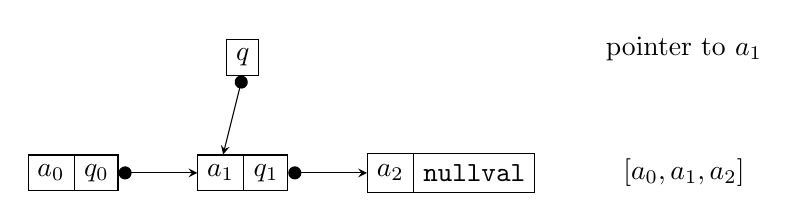
\begin{tikzpicture}[list/.style={rectangle split, rectangle split parts=2,
        draw, rectangle split horizontal}, >=stealth]
    
    \pause[1] \node[list] (A) {$a_0$ \nodepart{two} $q_0$};
    \pause[1] \node[list] (B) [right=of A] {$a_1$ \nodepart{two} $q_1$};
    \pause[1] \node[list] (C) [right=of B] {$a_2$ \nodepart{two} \texttt{nullval}};
    \pause[2] \node[draw, rectangle] (D) [above=of B] {$q$};
    \pause[1] \node (E) [right=of C] {$[a_0,a_1,a_2]$};
    \pause[2] \node (F) [above=of E] {pointer to $a_1$};
    \pause[1] \draw[*->] let \p1 = (A.east), \p2 = (A.center) in (\x1,\y2) -- (B);
    \pause[1] \draw[*->] let \p1 = (B.east), \p2 = (B.center) in (\x1,\y2) -- (C);
    \pause[2] \draw[*->] (D.south) -- ([xshift=-0.25cm]B.north);
  \end{tikzpicture}
  \vfill
  \begin{lstlisting}[language=Coq]
Fixpoint list_rep {A} (l:list A) (p:val) : mpred :=
  match l with
    | [ ] => emp
    | ai::l' => EX pi:val, cell_rep ai pi p * list_rep l' pi
  end.
  \end{lstlisting}
  \vfill
  \onslide<2>{\begin{center}
    \color{mDarkRed}$q=q0?$
  \end{center}}
\end{frame}

\begin{frame}[fragile]{Augmented Type}

  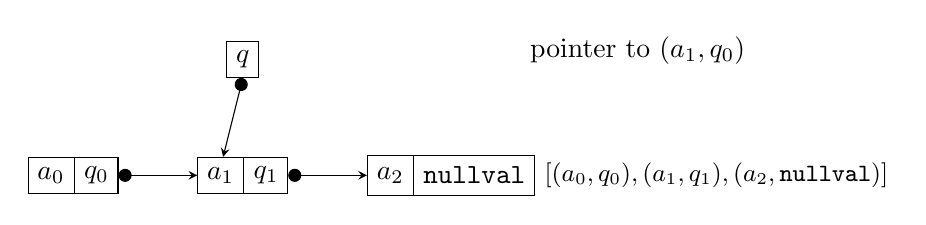
\begin{tikzpicture}[list/.style={rectangle split, rectangle split parts=2,
        draw, rectangle split horizontal}, >=stealth]
    
    \node[list] (A) {$a_0$ \nodepart{two} $q_0$};
    \node[list] (B) [right=of A] {$a_1$ \nodepart{two} $q_1$};
    \node[list] (C) [right=of B] {$a_2$ \nodepart{two} \texttt{nullval}};
    \node[draw, rectangle] (D) [above=of B] {$q$};
    \node (E) [right=of C,xshift=-1cm] {\small$[(a_0,q_0),(a_1,q_1),(a_2,\texttt{nullval})]$};
    \node (F) [above=of E,xshift=-1cm] {pointer to $(a_1,q_0)$};
    \draw[*->] let \p1 = (A.east), \p2 = (A.center) in (\x1,\y2) -- (B);
    \draw[*->] let \p1 = (B.east), \p2 = (B.center) in (\x1,\y2) -- (C);
    \draw[*->] (D.south) -- ([xshift=-0.25cm]B.north);
  \end{tikzpicture}
  \vfill
 \begin{lstlisting}[language=Coq]
Fixpoint list_rep {A} (l:concrete_list A) (p:val) : mpred :=
  match l with
    | [ ] => emp
    | (ai,pi)::l' => cell_rep ai pi p * list_rep l' pi
  end.
 \end{lstlisting}
 \vfill
 \begin{center}
   \phantom{\color{mDarkRed}$q=q0?$}
  \end{center}
\end{frame}


\begin{frame}{Augmented \btrees\ types}
  \cursorsep
  \begin{tikzpicture}[remember picture, overlay,%
      ]
      \node[anchor=north west,
      xshift=1.8cm,
      yshift=-5cm] 
      at (current page.north west) (S) {};
      \draw[draw=black,fill=black] ([yshift=-0.2cm]S) rectangle ++(0.05cm,3cm);
 \end{tikzpicture}
\end{frame}

\begin{frame}[fragile]{Augmented \btrees\ types}

  \begin{lstlisting}[language=Coq,basicstyle=\scriptsize,escapeinside={<@}{@>}]
(* Btree Types *)
Inductive entry (X:Type): Type :=
     | keyval: key -> V -> X -> entry X
     | keychild: key -> node X -> entry X
with node (X:Type): Type :=
     | btnode: option(node X)-> listentry X-> bool-> bool-> bool-> <@\color{mDarkRed}\texttt{X}@> -> node X
with listentry (X:Type): Type :=
     | nil: listentry X
     | cons: entry X -> listentry X -> listentry X.

Definition cursor (X:Type): Type := list (node X * index). (* ancestors and index *)
Definition relation (X:Type): Type := node X * X.  (* root and address *)
  \end{lstlisting}
  \vfill
  \begin{lstlisting}[language=Coq]
Definition concrete_tree : Type := node val.
Definition abstract_tree : Type := node unit.
  \end{lstlisting}

  
\end{frame}

\begin{frame}[fragile]{A B+Tree with Cursors functional model}

  \begin{lstlisting}[language=Coq,basicstyle=\scriptsize]
(* takes a PARTIAL cursor, n next node (pointed to by the cursor)
   and goes down to the first key *)
Fixpoint moveToFirst {X:Type} (n:node X) (c:cursor X) (level:nat): cursor X :=
  match n with
    btnode ptr0 le isLeaf First Last x =>
    match isLeaf with
    | true => (n,ip 0)::c
    | false => match ptr0 with
               | None => c      (* not possible, isLeaf is false *)
               | Some n' => moveToFirst n' ((n,im)::c) (level+1)
               end
    end
  end.
\end{lstlisting}
  
\end{frame}

\begin{frame}[fragile]{Specifying a C program with VST}
 \begin{lstlisting}[language=Coq,basicstyle=\small]
Definition RL_MoveToNext_spec : ident * funspec :=
  DECLARE _RL_MoveToNext
  WITH c:cursor val, pc:val, r:relation val, numrec:nat
  PRE[ _cursor OF tptr tcursor ]
    PROP(complete_cursor c r)
    LOCAL(temp _cursor pc)
    SEP(relation_rep r numrec; cursor_rep c r pc)
  POST[ tvoid ]
    PROP()
    LOCAL()
    SEP(relation_rep r numrec; cursor_rep (RL_MoveToNext c r) r pc).
 \end{lstlisting}
 \vfill
 \begin{center}
   \hoare{P}{S}{Q}
 \end{center}
 \begin{tikzpicture}[remember picture, overlay,%
      ]
      \node[anchor=north west,
      xshift=0.5cm,
      yshift=-1.7cm] 
      at (current page.north west) (S) {\prog{$S$\phantom{$PQ$}}};
      \draw[draw=prog,fill=prog] ([yshift=-0.2cm]S) rectangle ++(0.1cm,0.4cm);
 \end{tikzpicture}
 \begin{tikzpicture}[remember picture, overlay,%
      ]
      \node[anchor=north west,
      xshift=0.5cm,
      yshift=-3.35cm] 
      at (current page.north west) (P) {\spec{$P$}\phantom{$SQ$}};
      \draw[draw=spec,fill=spec] ([yshift=-0.9cm]P) rectangle ++(0.1cm,1.8cm);
 \end{tikzpicture}
 \begin{tikzpicture}[remember picture, overlay,%
      ]
      \node[anchor=north west,
      xshift=0.5cm,
      yshift=-5.3cm] 
      at (current page.north west) (Q) {\spec{$Q$}\phantom{$SP$}};
      \draw[draw=spec,fill=spec] ([yshift=-0.9cm]Q) rectangle ++(0.1cm,1.8cm);
    \end{tikzpicture}
\end{frame}


\begin{frame}[fragile]{Proving a C program correct with VST}
  \begin{lstlisting}[language=C, basicstyle=\scriptsize\ttfamily]
static BtNode* createNewNode(Bool isLeaf, Bool First, Bool Last) {
    BtNode* newNode;
    newNode = (BtNode*) surely_malloc(sizeof (BtNode));
    if (newNode == NULL) {
      return NULL; }
    newNode->numKeys = 0;
    newNode->isLeaf = isLeaf;
    newNode->First = First;
    newNode->Last = Last;
    newNode->ptr0 = NULL;
    return newNode; }
  \end{lstlisting}
  \begin{lstlisting}[language=Coq, basicstyle=\tiny]
Definition createNewNode_spec : ident * funspec :=
  DECLARE _createNewNode
  WITH isLeaf:bool, First:bool, Last:bool
  PRE [ _isLeaf OF tint, _First OF tint, _Last OF tint ]
    PROP ()
    LOCAL (temp _isLeaf (Val.of_bool isLeaf);
           temp _First (Val.of_bool First);
           temp _Last (Val.of_bool Last))
    SEP ()
  POST [ tptr tbtnode ]
    EX p:val, PROP ()
    LOCAL (temp ret_temp p)
    SEP (btnode_rep (empty_node isLeaf First Last p)).
  \end{lstlisting}

\end{frame}

{ % all template changes are local to this group.
  \addtocounter{framenumber}{1}
    \setbeamertemplate{navigation symbols}{}
    \begin{frame}[standout]
      \begin{tikzpicture}[remember picture,overlay]
        \node[at=(current page.center)] {
          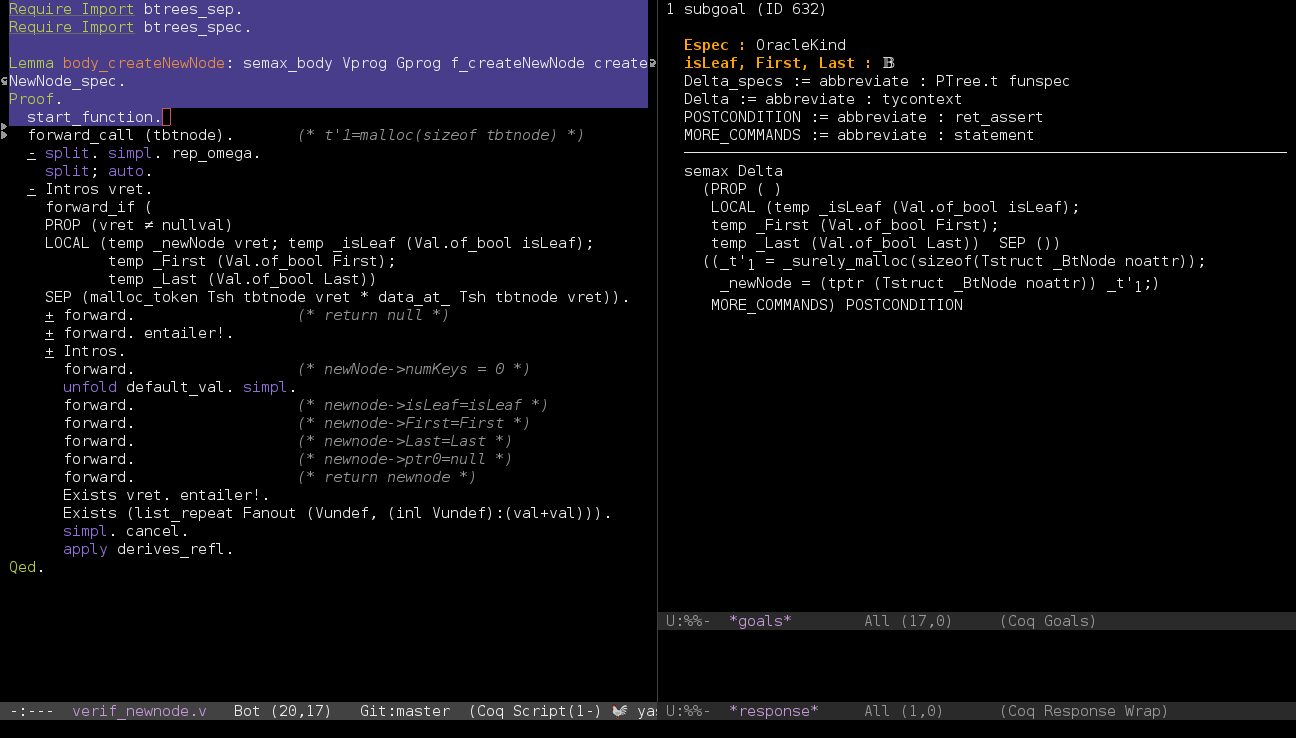
\includegraphics[width=\paperwidth]{proof1.png}
        };%
        \node[anchor=north west, xshift=6.4cm, yshift=-3.3cm] at (current page.north west) (S) {};
        \draw[draw=prog,fill=prog] (S) rectangle ++(0.1cm,0.65cm);
        \node[anchor=north west, xshift=6.4cm, yshift=-2.6cm] at (current page.north west) (P) {};
        \draw[draw=spec,fill=spec] (P) rectangle ++(0.1cm,0.95cm);
        \node[anchor=north west, xshift=8.4cm, yshift=-3.45cm] at (current page.north west) (Q) {};
        \draw[draw=spec,fill=spec] (Q) rectangle ++(1.4cm,0.1cm);
 \end{tikzpicture}
    \end{frame}
    \begin{frame}[standout]
      \begin{tikzpicture}[remember picture,overlay]
        \node[at=(current page.center)] {
          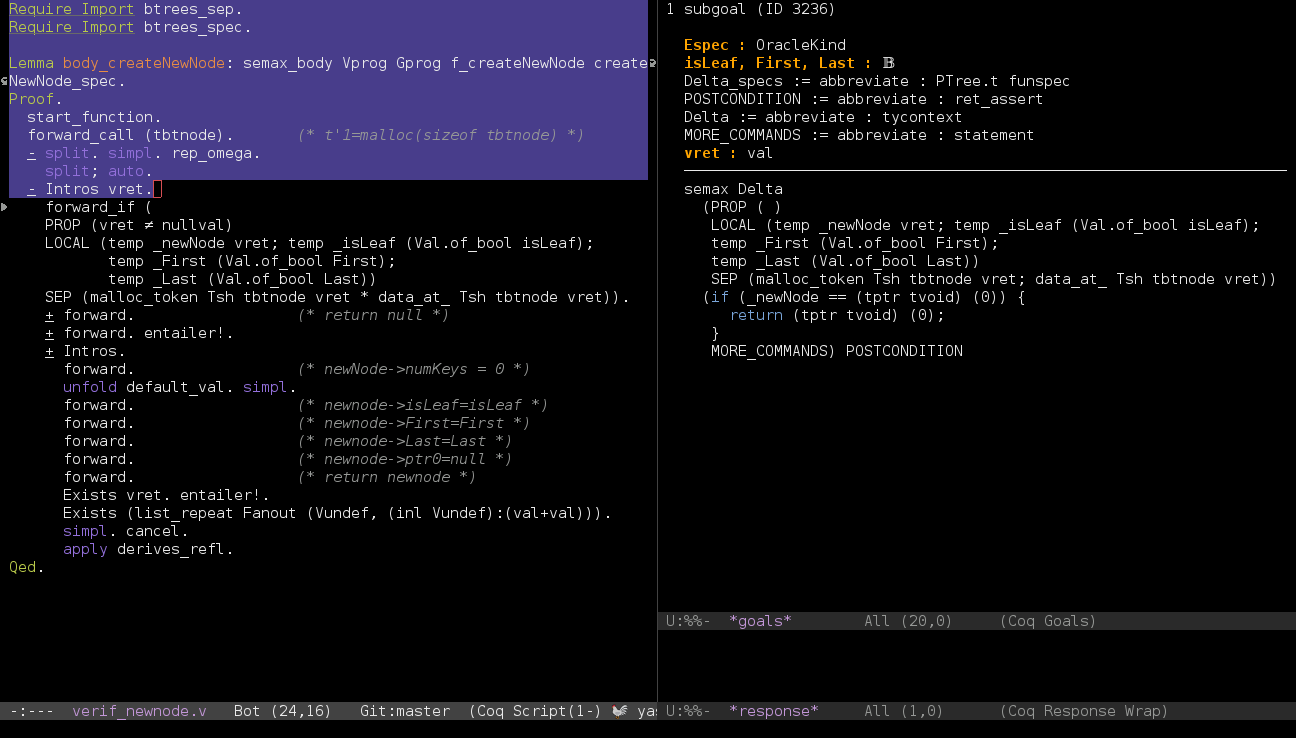
\includegraphics[width=\paperwidth]{proof2.png}
        };%
        \node[anchor=north west, xshift=6.4cm, yshift=-4cm] at (current page.north west) (S) {};
        \draw[draw=prog,fill=prog] (S) rectangle ++(0.1cm,0.75cm);
        \node[anchor=north west, xshift=6.4cm, yshift=-3.2cm] at (current page.north west) (P) {};
        \draw[draw=spec,fill=spec] (P) rectangle ++(0.1cm,1.3cm);
        \node[anchor=north west, xshift=8.4cm, yshift=-4.15cm] at (current page.north west) (Q) {};
        \draw[draw=spec,fill=spec] (Q) rectangle ++(1.4cm,0.1cm);
      \end{tikzpicture}
    \end{frame}
        \begin{frame}[standout]
      \begin{tikzpicture}[remember picture,overlay]
        \node[at=(current page.center)] {
          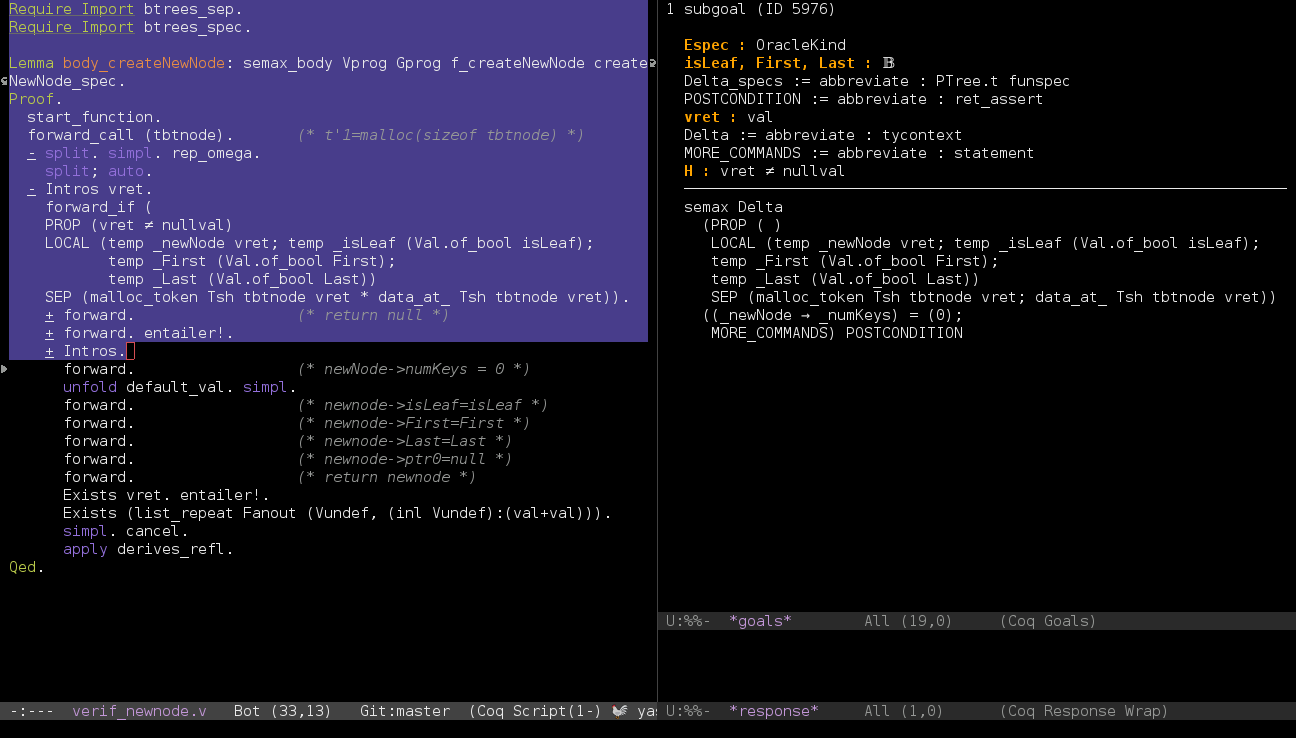
\includegraphics[width=\paperwidth]{proof3.png}
        };%
        \node[anchor=north west, xshift=6.4cm, yshift=-3.8cm] at (current page.north west) (S) {};
        \draw[draw=prog,fill=prog] (S) rectangle ++(0.1cm,0.4cm);
        \node[anchor=north west, xshift=6.4cm, yshift=-3.35cm] at (current page.north west) (P) {};
        \draw[draw=spec,fill=spec] (P) rectangle ++(0.1cm,1.3cm);
        \node[anchor=north west, xshift=8.4cm, yshift=-3.95cm] at (current page.north west) (Q) {};
        \draw[draw=spec,fill=spec] (Q) rectangle ++(1.4cm,0.1cm);
      \end{tikzpicture}
    \end{frame}
    \begin{frame}[standout]
      \begin{tikzpicture}[remember picture,overlay]
        \node[at=(current page.center)] {
          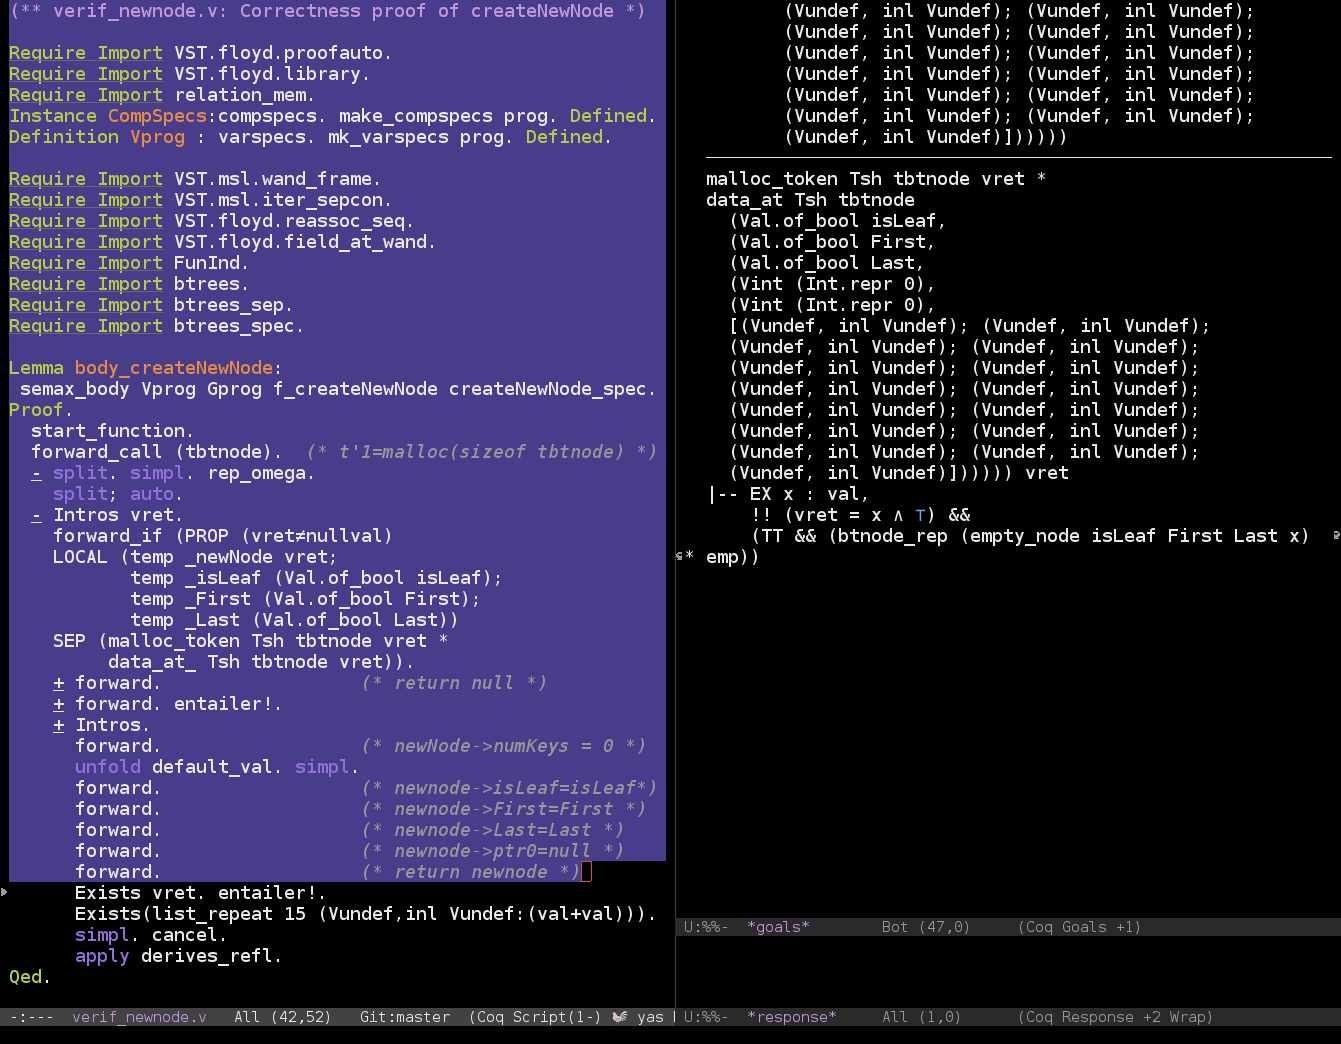
\includegraphics[width=\paperwidth]{proof4.png}
        };%
        \node[anchor=north west, xshift=6.4cm, yshift=-5.05cm] at (current page.north west) (Q) {};
        \draw[draw=spec,fill=spec] (Q) rectangle ++(0.1cm,0.8cm);
        \node[anchor=north west, xshift=6.4cm, yshift=-4.2cm] at (current page.north west) (P) {};
        \draw[draw=spec,fill=spec] (P) rectangle ++(0.1cm,3cm);
      \end{tikzpicture}
    \end{frame}
    \begin{frame}[standout]
      \begin{tikzpicture}[remember picture,overlay]
        \node[at=(current page.center)] {
          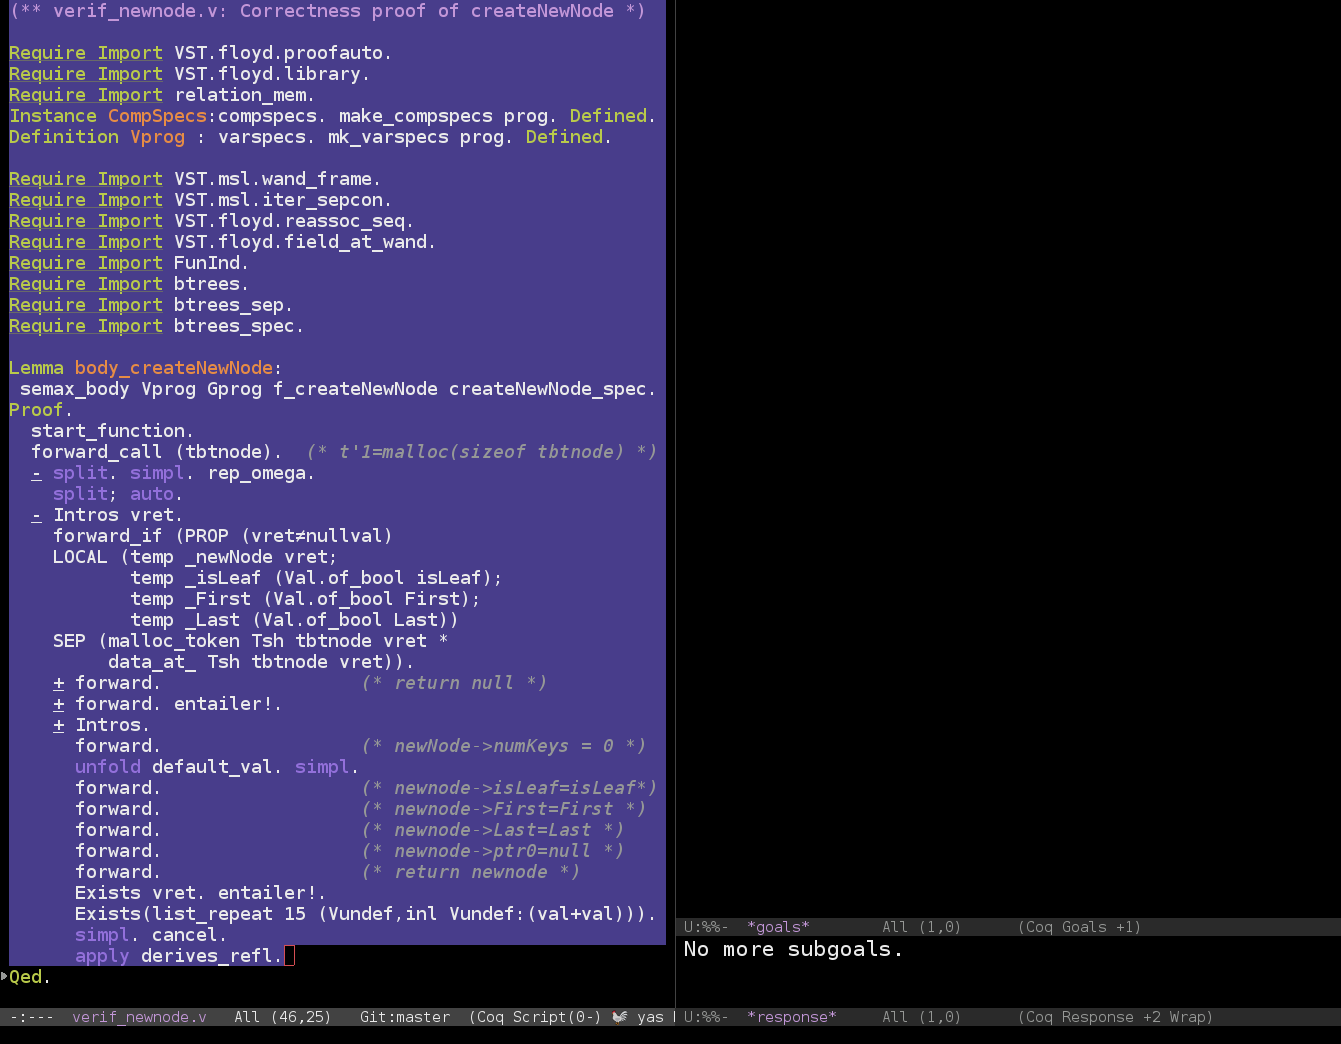
\includegraphics[width=\paperwidth]{proof5.png}
        };
      \end{tikzpicture}
    \end{frame}

}

\begin{frame}[fragile]{Bugs of the Original Implementation}
  \begin{lstlisting}[language=C]
if (node->entries[targetIdx].key == key)
  \end{lstlisting}
  \vfill
  \bugcursor
  % buildnig cursor for non key values
  % wrong array access
  % wrong complexity
  % others
\end{frame}

\section{Future Work}
\begin{frame}{Results}

  \begin{exampleblock}{Finished Proofs}
    All 27 C functions are specified and proved using VST.
  \end{exampleblock}
  \vfill
  \begin{alertblock}{Remaining Proofs}
    Many theorems about the \textbf{functional} model.
  \end{alertblock}
  \vfill
  \begin{itemize}
  \item 1 kloc functional model and related lemmas
  \item 1 kloc representation predicates and functions specifications
  \item 5 kloc VST proofs
  \end{itemize}
  
\end{frame}

\begin{frame}{Conclusion}
  \begin{block}{Contribution}
    We now have
    \begin{itemize}
    \item A modified C library for \btrees\ with Cursors.
    \item A Coq functional model for \btrees\ with Cursors.
    \item A VST correctness proof relating the two.
    \end{itemize}
    {\scriptsize\texttt{https://github.com/PrincetonUniversity/DeepSpecDB}}
  \end{block}
  \vfill
  \begin{block}{Future Work}
    \begin{itemize}
    \item Prove the remaining Lemmas.
    \item Prove correctness of the entire data-structure.
    \item Concurrent database.
    \end{itemize}
  \end{block}
  
\end{frame}

\end{document}
